\chapter{Extraction Method Based on ILP Machine Learning}
\graphicspath{{../img/ch60/}}


\section{Introduction}
Automated semantic annotation (SA) is considered to be one of the most important elements in the evolution of the Semantic Web. Besides that, SA can provide great help in the process of data and information integration and it could also be a basis for intelligent search and navigation.

In this paper we present main results and reflections of our ongoing PhD project, a method for classical and semantic information extraction and annotation of texts, which is based on a deep linguistic analysis and Inductive Logic Programming (ILP). This approach is quite novel because it directly combines deep linguistic parsing with machine learning (ML). This combination and the use of ILP as a ML engine have following benefits: Manual selection of learning features is not needed. 
The learning procedure has full available linguistic information at its disposal and it is capable to select relevant parts itself. Extraction rules learned by ILP can be easily visualized, understood and adapted by human.

A description, implementation and initial evaluation of the method are the main contributions of the paper.









\section{Implementation}
Here we just briefly describe implementation of our system. The system consists of several modules, all integrated in GATE as processing resources.

\subsection{TectoMT Wrapper (Linguistic Analysis)} 

TectoMT wrapper is a GATE component (processing resource), which takes the text of a GATE document, sends it to TectoMT linguistic analyzers, parses the results and converts the results to the form of GATE annotations.

Because TectoMT has to run as a separate process (it is implemented in Perl) and the initialization of TectoMT analyzers usually takes significant amount of time it would be very inefficient to start a new TectoMT instance for each document. Therefore the implementation currently offers two modes of execution: batch (TectoMTBatchAnalyser) and online (TectoMTOnlineAnalyser).

The batch mode is implemented similarly to the Batch Learning PR\footnote{\url{http://gate.ac.uk/userguide/sec:ml:batch-learning-pr}}. During the execution as a part of a corpus pipeline it only accumulates documents and the whole work is done as a batch when the last document is encountered. This also implies that TectoMTBatchAnalyser has to be the last PR in the pipeline because it produces no output in the time of execution (except for the last document). 

Client-server model of implementation is used in the online mode. A separate TectoMT server process is started at the time of initialization and GATE documents are processed in ordinary way at the time of execution. This means that (similarly to the previous case) each document is converted to the TectoMT readable format, sent to TectoMT and the result is converted back to GATE. The online mode of execution is a bit slower than the batch mode because additional time is spent on client-server communication (XML-RPC\footnote{\url{http://www.xmlrpc.com/}}).



\subsection{PDT Annotations in GATE} \label{sec:pdt_in_gate}

Although GATE annotations are just highlighted pieces of text it is possible to use them to encode dependency tree structures. It is possible because each GATE annotation has a unique identifier (ID) and an arbitrary set of features (name-value pairs) can be assigned to it. The way how the PDT dependency trees are encoded in GATE is in fact the same as in the GATE wrapper for the Stanford Parser\footnote{\url{http://gate.ac.uk/userguide/sec:parsers:stanford}}. 

Three main constructs are used to capture an arbitrary configuration of a linguistic dependency tree:


\begin{description}
	\item[tree nodes] (usually corresponding to words (tokens) of a sentence)
	\item[edges] (dependency relations between nodes)
	\item[node attributes] (connected linguistic features like POS, gender, tense, case, etc.)
\end{description}

These constructs are encoded in GATE in the following way: tree nodes correspond to token annotations, node attributes are saved as token annotation features and edges are encoded as another special kind of annotations.

Two kinds of token annotations are used to represent two kinds of trees and tree nodes. ``Token'' annotation type is used for analytical tree nodes and ``tToken'' for tectogrammatical tree nodes.

Four kinds of edges (dependencies) are implemented by the TectoMT wrapper: analytical dependencies, tectogrammatical dependencies, aux.rf (auxiliary reference) and lex.rf (main lexical reference). The last two kinds (aux.rf and lex.rf) are used to connect tectogrammatical and analytical nodes. The implementation differs according to the cardinality of a dependency type. The first three kinds are of the cardinality one-to-many (one parent node can have many children nodes) and the last one (lex.rf) if of the cardinality one-to-one (one parent node has at most one child). Because of that lex.rf edges can be stored as features (with the name ``lex.rf'') of ``tToken'' annotations. Note that a GATE annotation feature can only have one value per annotation. In this case the annotation ID of the referenced ``Token'' annotation (referenced analytical node) is the value of the lex.rf feature.

One-to-many dependencies are stored as separate annotations (type names: ``aDependency'', ``tDependency'', ``aux.rf'') with a single feature called ``args''. Values of this feature are of Java type List<Integer> (list of integers). The list always contains just two items. The first one is the annotation ID of the parent annotation; the second one is the ID of the child annotation. Instead of using one list feature, two simple features (like ``arg1'', ``arg2'' or ``parentID'', ``childID'') could be used, but the implementation is consistent with the wrapper for the Stanford Parser (using the single list feature ``args''), thus PDT dependencies are compatible with Stanford dependencies in GATE.

It is not simple to demonstrate the GATE representation of the dependencies in a static printed form; we can only show a GATE screenshot (Figure~\ref{fig:PDT_GATE}) that partly illustrates that.


\begin{figure}
	\centering
		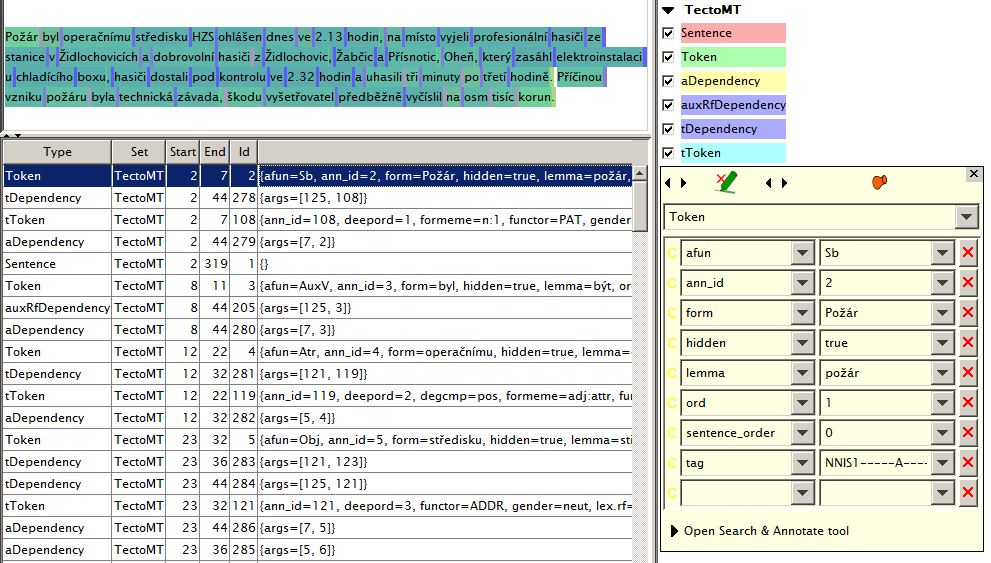
\includegraphics[width=0.7\hsize]{PDT_GATE}
	\caption{PDT annotations in GATE (screenshot).}
	\label{fig:PDT_GATE}
\end{figure}



\subsection{ILP Wrapper (Machine Learning)}
After a human annotator have annotated several documents with desired target annotations, machine learning takes place. 
This consists of two steps: 
\begin{enumerate}
	\item learning of extraction rules from the target annotations and
	\item application of the extraction rules on new documents.
\end{enumerate}
In both steps the linguistic analysis has to be done before and in both steps background knowledge (a logical database of facts) is constructed from linguistic structures of documents that are being processed. We call the process of background knowledge construction as \emph{ILP serialization}; more details are presented below in Section~\ref{sec:ilp_serialization}.

After the ILP serialization is done, in the learning case, positive and negative examples are constructed from target annotations and the machine learning ILP inductive procedure is executed to obtain extraction rules.

In the application case a Prolog system is used to check if the extraction rules entail any of target annotation candidates.


%Learning / application
%\\1.	serialization -> learning in ILP
%\\2.	serialization -> application in ILP


The learning examples and annotation candidates are usually constructed from all document tokens (and we did so in the present solution), but it can be optionally changed to any other textual unit, for example only numerals or tectogrammatical nodes (words with lexical meaning) can be selected. This can be done easily with the help of \emph{Machine Learning PR} (LM PR) from GATE\footnote{\emph{Machine Learning PR} is an old GATE interface for ML and it is almost obsolete but in contrast to the new \emph{Batch Learning PR} the LM PR is easy to extend for a new ML engine.}.

ML PR provides an interface for exchange of features (including target class) between annotated texts and propositional learners in both directions -- during learning as well as during application. We have used ML PR and developed our \emph{ILP Wrapper} for it. The implementation was a little complicated because complex linguistic structures cannot be easily passed as propositional features, so in our solution we use the ML PR interface only for exchange of the class attribute and annotation id and we access the linguistic structures directly in a document.



\subsection{ILP Serialization} \label{sec:ilp_serialization}

In this section details about conversion of linguistic trees to ILP background knowledge (a Prolog logical database of facts) will be presented. Although the construction is quite strait forward it is worth describing because it makes it easier to understand the extraction rules found by the ILP learning procedure. 

As mentioned in Section~\ref{sec:pdt_in_gate}: three main constructs are used to capture an arbitrary configuration of a dependency linguistic tree: nodes, edges and node attributes. During the process of ILP Serialization these constructs are rendered to Prolog in following way. 

A unique identifier (node ID) is generated for every tree node. The identifier is based on document name and GATE annotation ID (sentence order and node deep order are used outside of GATE, see PML$\rightarrow$RDF transformation in Section~\ref{sec:pml_to_rdf}.) These node IDs correspond to simple atoms and they represent tree nodes in the fact database. A node type (used by the ILP learning algorithm) is assigned to a node ID by predicates \texttt{Token(NodeID)} for analytical tree nodes and \texttt{tToken(NodeID)} for tectogrammatical tree nodes.

Tree nodes are connected by edges using binary predicates of the form:

\texttt{dependency\_type\_name(ParentNodeID, ChildNodeID)}

\noindent Note that the parent (governor) node always occupies the first argument and the child (dependant) node the second one. Predicate name \emph{tDependency} is used for tectogrammatical dependencies and \emph{aDependency} for analytical ones. There are also special kinds of dependencies that connect tectogrammatical and analytical nodes: \emph{lex.rf} (main lexical reference) and \emph{aux.rf} (auxiliary reference), in these cases tectogrammatical node occupies the first argument and analytical the second.

Node attributes are assigned to node IDs by binary predicates of the form:

\texttt{attribute\_name(NodeID, AttributeValue)}

\noindent There are about thirty such predicates like \emph{t\_lemma} (tectogrammatical lemma), \emph{functor} (tectogrammatical functor), \emph{sempos} (semantic part of speech), \emph{negation}, \emph{gender}, etc. but minority of them is usually used in extraction rules.

Example of a serialized tectogrammatical tree is in Listing~\ref{lst:ilp_serialization} it is the same tree as in Figure~\ref{img:damage_tree}.


%%%%%%%%%%%%%%%%%%%%%%%%%%%%%%%%%%%%%%%%%%%%%%%%%%%%%%%%%%%%%%%%%%%%%%%%%%%%%%%%%%%%%
\begin{listing}[ht]
\begin{minted}[linenos, fontsize=\footnotesize,
               frame=lines]{prolog}
tToken(  id_jihomoravsky47443_243).
t_lemma( id_jihomoravsky47443_243, 'být'). %to be
functor( id_jihomoravsky47443_243, 'PRED').
sempos(  id_jihomoravsky47443_243, 'v').
tDependency( id_jihomoravsky47443_243, id_jihomoravsky47443_238).
tToken(  id_jihomoravsky47443_238).
t_lemma( id_jihomoravsky47443_238, ','). %comma
functor( id_jihomoravsky47443_238, 'APPS').
sempos(  id_jihomoravsky47443_238, 'n.denot').
gender(  id_jihomoravsky47443_238, 'nr').
tDependency( id_jihomoravsky47443_238, id_jihomoravsky47443_237).
tToken(  id_jihomoravsky47443_237).
t_lemma( id_jihomoravsky47443_237, 'vyčíslit'). %to quantify
functor( id_jihomoravsky47443_237, 'PAT').
sempos(  id_jihomoravsky47443_237, 'v').
tDependency( id_jihomoravsky47443_237, id_jihomoravsky47443_245).
tToken(  id_jihomoravsky47443_245).
t_lemma( id_jihomoravsky47443_245, 'předběžně'). %preliminarily
functor( id_jihomoravsky47443_245, 'MANN').
sempos(  id_jihomoravsky47443_245, 'adv.denot.grad.nneg').
tDependency( id_jihomoravsky47443_237, id_jihomoravsky47443_244).
tToken(  id_jihomoravsky47443_244).
t_lemma( id_jihomoravsky47443_244, 'vyšetřovatel'). %investigator
functor( id_jihomoravsky47443_244, 'ACT').
sempos(  id_jihomoravsky47443_244, 'n.denot').
gender(  id_jihomoravsky47443_244, 'anim').
tDependency( id_jihomoravsky47443_237, id_jihomoravsky47443_240).
tToken(  id_jihomoravsky47443_240).
t_lemma( id_jihomoravsky47443_240, 'osm'). %eight
functor( id_jihomoravsky47443_240, 'PAT').
sempos(  id_jihomoravsky47443_240, 'n.quant.def').
gender(  id_jihomoravsky47443_240, 'nr').
tDependency( id_jihomoravsky47443_240, id_jihomoravsky47443_242).
tToken(  id_jihomoravsky47443_242).
t_lemma( id_jihomoravsky47443_242, 'tisíc'). %thousand
functor( id_jihomoravsky47443_242, 'RSTR').
sempos(  id_jihomoravsky47443_242, 'n.quant.def').
gender(  id_jihomoravsky47443_242, 'inan').
tDependency( id_jihomoravsky47443_242, id_jihomoravsky47443_247).
tToken(  id_jihomoravsky47443_247).
t_lemma( id_jihomoravsky47443_247, 'koruna'). %crown
functor( id_jihomoravsky47443_247, 'MAT').
sempos(  id_jihomoravsky47443_247, 'n.denot').
gender(  id_jihomoravsky47443_247, 'fem').
tDependency( id_jihomoravsky47443_237, id_jihomoravsky47443_246).
tToken(  id_jihomoravsky47443_246).
t_lemma( id_jihomoravsky47443_246, 'škoda'). %damage
functor( id_jihomoravsky47443_246, 'PAT').
sempos(  id_jihomoravsky47443_246, 'n.denot').
gender(  id_jihomoravsky47443_246,'fem').
\end{minted}
\caption{ILP serialization example}
\label{lst:ilp_serialization}
\end{listing}
%%%%%%%%%%%%%%%%%%%%%%%%%%%%%%%%%%%%%%%%%%%%%%%%%%%%%%%%%%%%%%%%%%%%%%%%%%%%%%%%%%%%%




\subsection{Connecting Linear GATE Annotations with Tree Nodes}


\subsection{Root/Subtree Preprocessing/Postprocessing}
Sometimes annotations span over more than one token. This situation complicates the process of machine learning and this situation is often called as ``chunk learning''. Either we have to split a single annotation to multiple learning instances and after application we have to merge them back together, or we can change the learning task from learning annotated tokens to learning borders of annotations (start tokens and end tokens). The later approach is implemented in GATE in \emph{Batch Learning PR} in the `SURROUND' mode.

We have used another approach to solve this issue. Our approach is based on syntactic structure of a sentence and we call it ``root/subtree preprocessing/postprocessing''. The idea is based on the observation that tokens of a multi-token annotation usually have a common parent node in a syntactic tree. So we can
\begin{enumerate}
	\item extract the parent nodes (in dependency linguistics this node is also a token and it is usually one of the tokens inside the annotation), 
	\item learn extraction rules for parent nodes only and 
	\item span annotations over the whole subtrees of root tokens found during the application of extraction rules.
\end{enumerate}
We call the first point as \emph{root preprocessing} and the last point as \emph{subtree postprocessing}. We have successfully used this technique for the `damage' task of our evaluation corpus (See Section~\ref{sec:evaluation} for details.)

\subsection{Semantic Interpretation}
\label{sec:SemanticInterpretation}
Information extraction can solve the task ``how to get documents annotated'', but as we aim on the semantic annotation, there is a second step of ``semantic interpretation'' that has to be done. In this step we have to interpret the annotations in terms of a standard ontology. On a very coarse level this can be done easily. Thanks to GATE ontology tools \citep{Bon04b} we can convert all the annotations to ontology instances with a quite simple JAPE \citep{Cunningham00jape:a} rule, which takes the content of an annotation and saves it as a label of a new instance or as a value of some property of a shared instance. For example in our case of traffic and fire accidents, there will be a new instance of an accident class for each document and the annotations would be attached to this instance as values of its properties. Thus from all annotations of the same type, instances of the same ontology class or values of the same property would be constructed. This is very inaccurate form of semantic interpretation but still it can be useful. It is similar to the GoodRelation \citep{DBLP:conf/ekaw/Hepp08} design principle of \emph{incremental enrichment}\footnote{
\url{http://www.ebusiness-unibw.org/wiki/Modeling_Product_Models#Recipe:_.22Incremental_Enrichment.22}
}:
\begin{quote}
``...you can still publish the data, even if not yet perfect. The Web will do the rest -- new tools and people.''	
\end{quote}

But of course we are not satisfied with this fashion of semantic interpretation and we plan to further develop the semantic interpretation step as a sophisticated ``annotation $\rightarrow$ ontology'' transformation process that we have proposed in one of our previous works \citep{biblio:DeVoComputingaggregations2008}.

\subsection{How to Download}
The project website\footnote{\url{http://czsem.berlios.de}} provides several ways how to get all the presented tools running. A platform independent installer, Java binaries and source codes are provided under the GPL license.


\section{Evaluation}
\label{sec:evaluation}

\subsection{Dataset}
We have evaluated our state of the art solution on a small dataset that we use for development. It is a collection of 50 Czech texts that are reporting on some accidents (car accidents and other actions of fire rescue services). These reports come from the web of Fire rescue service of Czech Republic\footnote{\url{http://www.hzscr.cz/hasicien/}}. The labeled corpus is publically available on the web of our project\footnote{\url{http://czsem.berlios.de/}}.
The corpus is structured such that each document represents one event (accident) and several attributes of the accident are marked in text. For the evaluation we selected two attributes of different kind. The first one is `damage' -- an amount (in CZK - Czech Crowns) of summarized damage arisen during a reported accident. The second one is `injuries', it marks mentions of people injured during an accident. These two attributes differ. Injuries annotations always cover only a single token, while damage annotations usually consist of two or three tokens -- one or two numerals express the amount and one extra token is for currency.

These two attributes differ in two directions:
\begin{enumerate}
	\item Injuries annotations always cover only a single token while damage usually consists of two or three tokens - one or two numerals express the amount and one extra token is for currency.
	\item The complexity of the marked information (and the difficulty of the corresponding extraction task) differs slightly. While labeling of all money amounts in the corpus will result in 75\% accuracy for damage annotations, in the case of injured persons mentions there are much more possibilities and indications are more spread in context.
\end{enumerate}

\subsection{Comparison with Paum classifier}
To compare our solution with other alternatives we took the Paum propositional learner from GATE \citep{Li:Paum}. The quality of propositional learning from texts is strongly dependent on the selection of right features. We obtained quite good results with features of a window of two preceding and two following token lemmas and morphological tags. The precision was further improved by adding the feature of \emph{analytical function} from the syntactic parser (see the last row of Table~\ref{tab:EvaluationResults}).

Because we did not want to invest much time to this and the feature setting of the Paum learner was quite simple (a window of two preceding and following token lemmas and morphological tags). We admit that looking for better features could further improve the results of the Paum learner.

\subsection{Cross validation}
We used the 10-fold cross validation in the evaluation. Thanks to this technique the evaluation is simple. After processing all the folds each document is processed with some of the ten learned models such that the particular document was not used in learning of that model, so all documents are unseen by the model applied on them. At the end we just compare the gold standard annotations with the learned ones in all documents.

\subsection{Results}


Results of a 10-fold cross validation are summarized in Table~\ref{tab:EvaluationResults}. We used standard information retrieval performance measures: precision, recall and $F_1$ measure and also theirs lenient variants (overlapping annotations are added to the correctly matching ones, the measures are the same if no overlapping annotations are present).

\begin{table}[t]
	\centering
			
\begin{tabular}{|l||r|r|r|r|r|r|r|}
\hline
\textbf{task/method} & \textbf{matching} & \textbf{missing} & \textbf{excessive} & \textbf{overlap} & \textbf{prec.}\% & \textbf{recall}\% & \textbf{F1.0}\%\\
\hline
\hline
\textbf{damage/ILP} & 14 & 0 & 7 & 6 & 51.85 & 70.00 & 59.57\\
\hline
\multicolumn{5}{|l|}{\textbf{damage/ILP -- lenient measures}} & 74.07 & 100.00 & 85.11\\
\hline
\textbf{dam./ILP-roots} & 16 & 4 & 2 & 0 & 88.89 & 80.00 & 84.21\\
\hline
\textbf{damage/Paum} & 20 & 0 & 6 & 0 & 76.92 & 100.00 & 86.96\\
\hline
\hline
\textbf{injuries/ILP} & 15 & 18 & 11 & 0 & 57.69 & 45.45 & 50.85\\
\hline
\textbf{injuries/Paum} & 25 & 8 & 54 & 0 & 31.65 & 75.76 & 44.64\\
\hline
\textbf{inj./Paum-afun} & 24 & 9 & 38 & 0 & 38.71 & 72.73 & 50.53\\
\hline
\end{tabular}
						
	\caption{Evaluation results }
	\label{tab:EvaluationResults}
	\vspace{-0.80cm}
\end{table}

In the first task (`damage') the methods obtained much higher scores then in the second (`injuries') because the second task is more difficult. In the first task also the root/subtree preprocessing/postprocessing improved results of ILP such that afterwards, annotation borders were all placed precisely. The ILP method had better precision and worse recall than the Paum learner but the $F_1$ score was very similar in both cases.

\subsubsection{Statistical Significance}
The term statistical significance refers to the result of a pair-wise comparison of learning engines using the corrected resampled (two tailed) T-Test \citep{Nadeau:2003:IGE:779909.779927}, which is suitable for cross validation based experiments. The Weka implementation\footnote{\url{http://www.cs.waikato.ac.nz/ml/weka/}} is used. Test significance is 0.05 in all cases.

\subsection{Examples of learned rules}

In Figure~\ref{fig:rules} we present some examples of the rules learned from the whole dataset. The rules demonstrate a connection of a target token with other parts of a sentence through linguistic syntax structures. For example the first rule connects a root numeral (\emph{n.quant.def}) of `damage' with a mention of `investigator' that stated the mount. In the last rule only a positive occurrence of the verb `injure' is allowed.

\begin{figure}
\begin{minted}[linenos,  fontsize=\footnotesize,
               frame=lines]{prolog}
%[Rule 1] [Pos cover = 14 Neg cover = 0]
damage_root(A) :- lex_rf(B,A), has_sempos(B,'n.quant.def'), tDependency(C,B),
   tDependency(C,D), has_t_lemma(D,'investigator').

%[Rule 2] [Pos cover = 13 Neg cover = 0]
damage_root(A) :- lex_rf(B,A), has_functor(B,'TOWH'), tDependency(C,B),
   tDependency(C,D), has_t_lemma(D,'damage').


%[Rule 1] [Pos cover = 7 Neg cover = 0]
injuries(A) :- lex_rf(B,A), has_functor(B,'PAT'), has_gender(B,anim),
   tDependency(B,C), has_t_lemma(C,'injured').

%[Rule 8] [Pos cover = 6 Neg cover = 0]
injuries(A) :- lex_rf(B,A), has_gender(B,anim), tDependency(C,B),
   has_t_lemma(C,'injure'), has_negation(C,neg0).
\end{minted}
	\caption{Examples of learned rules, Czech words are translated.}
	\label{fig:rules}
\end{figure}





Experience with human-designed rules.










\section{Conclusion and Future Work}
From our experiments can be seen that ILP is capable to find complex and meaningful rules that cover the intended information. But in terms of the performance measures the results are not better than those from a propositional learner. This is quite surprising observation because Czech is a language with free word order and we would expect much better results of the dependency approach than those of the position based approach, which was used by the propositional learner.

Our method is still missing an intelligent semantic interpretation procedure and it should be evaluated on bigger datasets (e.g. MUC, ACE, TAC, CoNLL) and other languages. So far we also do not provide a method for classical relation extraction (like e.g. in \citep{Bunescu:DependencyPaths}). In the present solution we deal with relations implicitly. The method has to be adapted for explicit learning of relations in the form of ``subject predicate object''.

Our method can also provide a comparison of linguistic formalisms and tools because on the same data we could run our method using different linguistic analyzers and compare the results.
